\documentclass[12pt,a4paper]{article}

% === PAQUETES === (((
\usepackage{amsmath}
\usepackage[shortlabels]{enumitem}
\usepackage{amsfonts}
\usepackage{ragged2e}
\usepackage{subfigure}
\usepackage{amssymb}
\usepackage{slashbox}
\usepackage{multirow}
\usepackage{multicol}
\usepackage{fontspec}
\usepackage{fullpage}
\usepackage{graphicx}
\usepackage{titlesec} 
% \usepackage{setspace}
\usepackage{dsfont}
% \usepackage{bookmark}
% )))

% === TIPOGRAFÍA === (((
\setmainfont[
  BoldFont       = bodonibi,
	ItalicFont     = Century modern italic2.ttf,
	BoldItalicFont = bodonibi,
	SmallCapsFont  = lmromancaps10-regular.otf
]{Century_modern.ttf}
% )))

% === COMANDOS === (((
\newcommand{\dis}{\displaystyle}
\newcommand{\qed}{\hspace{0.5cm}\rule{0.16cm}{0.4cm}}
\newcommand{\micita}[1]{\([\)\cite{#1}\(]\)}
\newcommand{\operator}[1]{\mathop{\vphantom{\sum}\mathchoice{ \vcenter{\hbox{\huge $#1$}} }
{\vcenter{ \hbox{\Large $#1$}} }{#1}{#1}}\displaylimits}
\newcommand{\suma}{\operator{ 
\includegraphics[scale=0.09]{IMAGENES/Sigma.png}} }
\DeclareSymbolFont{italics}{\encodingdefault}{\rmdefault}{m}{it}
\DeclareSymbolFontAlphabet{\mathit}{italics}
\ExplSyntaxOn
\int_step_inline:nnnn { `A } { 1 } { `Z }
 {  \exp_args:Nf \DeclareMathSymbol{\char_generate:nn{#1}{11}}{\mathalpha}{italics}{#1} }
\int_step_inline:nnnn { `a } { 1 } { `z } {  \exp_args:Nf \DeclareMathSymbol{\char_generate:nn{#1}{11}}{\mathalpha}{italics}{#1}}
\ExplSyntaxOff
% )))

% === SECCIONES === (((
\titleformat*{\section}{\large\normalfont\bfseries}
\titleformat*{\subsection}{\large\itshape \centering}
% \setcounter{secnumdepth}{0}
\renewcommand*{\contentsname}{\large\textbf{CONTENIDOS.}}
\usepackage[nottoc,numbib]{tocbibind}
\renewcommand{\refname}{REFERENCIAS.}
\renewcommand{\tablename}{Tabla}
\renewcommand{\figurename}{Figura}
% )))

% === PORTADA === (((
% \pagestyle{empty}
\newcommand{\portada}{
\addfontfeature{LetterSpace=-5}
  \begin{titlepage}
  \centering
  \begin{figure}
    \centering
    
\includegraphics[scale=0.5]{IMAGENES/logo_uaa.png}  
  \end{figure}
  {\bfseries\Large\MakeUppercase{\textit{Universidad Autónoma de Aguascalientes.}} \par}
  \vspace{1cm}
  {\Large Centro de Ciencias Básicas. \vspace{0.5cm}\\[2mm]
  Departamento de Matemáticas y Física.\vspace{0.5cm}\\[2mm]
  Licenciatura en Matemáticas Aplicadas.\vspace{0.5cm}\\[2mm]
  Práctica 6.\par}
  \vspace{1.5cm}
  {\bfseries\Huge Experimento de Young. \par} % title
  \vspace{1.5cm}
  {\itshape\Large Óptica. \\Prof. Mariana Alfaro Gómez.\par}
  % {\itshape\Large Variable Compleja I. \\Prof. Fausto Arturo Contreras Rosales.\par}
  % {\itshape\Large Métodos Numéricos II. \\Prof. Manuel Ramírez Aranda.\par}
  % {\itshape\Large Diseño de Experimentos. \\Prof. Angélica Hernández Quintero.\par}
  % {\itshape\Large Filosofía de la Investigación Científica. \\Prof. Jesús Mariano Rodríguez Muñoz.\par}
  \vfill
  % {\Large \textit{Por Erick I. Rodríguez Juárez.}\par}
		\begin{flushleft}
		\Large
		Alumnos:\\
		\textit{Carlos Francisco Guzmán Barba.}\\
		\textit{Erick Ignacio Rodríguez Juárez.}\\
		\textit{Manuel Alejandro Siller Landin.}
		\end{flushleft}
	% {}  % {\Large \textit{Por Erick I. Rodríguez Juárez.}\par}
  \vfill
		\begin{flushright}
		{\Large Realización: 2\(/\)05\(/\)22. \par} % date
		{\Large Entrega: 16\(/\)05\(/\)22. \par} % date
		\end{flushright}
  \end{titlepage} 
	% \thispagestyle{empty}
	% \doublespacing
	% \tableofcontents
	% \singlespacing
	% \newpage
} 
% )))

\begin{document}

\portada

\section{RESUMEN.} % (((
El propósito de este experimento fue determinar la velocidad de onda plana en el agua mediante el uso de un generador y cuba de ondas. Primeramente, obtuvimos los valores del período, empleando el uso del factor de amplificación de $F_A = 2\pm0.03$ para la cuba del laboratorio, dado que trabajamos constantemente con proyecciones de las ondas, dependiendo de la frecuencia generada, así como comparando los valores de la frecuencia medidos con los valores reales que podíamos leer del propio generador. En seguida generamos una estimación de dichos valores para estimar la velocidad la cual fue de $22.83\;cm/seg$ pues mediante una recta logramos determinar la relación entre ambos factores dado que a mayor frecuencia menor longitud de onda y, más aún, resaltar que permaneció constante aún cuando la frecuencia variaba en el agua.
% )))

\section{INTRODUCCIÓN.} % (((

\subsection{--- Marco Teórico ---} % (((
Las ondas son perturbaciones que viajan a través del espacio y del tiempo; existen varias formas de clasificarlas, ya sea de acuerdo a su forma, dirección o dimensión de propagación, entre otras, pero una de las principales es según su naturaleza, las cuales pueden ser: \textit{electromagnéticas}, donde tales ondas no requieren un medio para transportarse, por ejemplo, la luz o las ondas de radio; y \textit{mecánicas}, en donde necesariamente dependen de un medio para propagarse, como una ola sobre el agua o las ondas de sonido. El modo más simple y práctico de ver este tipo de ondas es en las denominadas “ondas planas”, las cuales consisten en ondas que se mueven en una sola dirección a lo largo del espacio a través del tiempo. En esta práctica nos enfocamos solamente a este tipo de ondas (planas), las cuales dependían de un medio para moverse (mecánicas). \\[2mm]
Para poder describir completamente las ondas, se han definido cualidades específicas que permiten caracterizar el movimiento de ellas. Sin embargo, para este tipo de experimento se prestó especial atención a sólo algunas de estas características, las cuales se definen a continuación:
\begin{enumerate}
	\item Longitud de onda (\(\lambda\)): es la distancia que existe entre dos puntos equivalentes (repeticiones de la forma) de la onda; su magnitud usual es en metros (\(m\)), pero para fines prácticos la manejaremos en centímetros (\(cm\)).
	\item Período (\(T\)): también llamado “período de oscilación”, es el tiempo que tardan los elementos de la onda en recorrer una longitud de onda completa; se mide en segundos (\(s\)).
	\item Frecuencia (\(f\)): es el inverso del período, nos dice el número de oscilaciones por unidad de tiempo, esto es
		\begin{equation}
			f = \dfrac{1}{T}.
			\label{eq:frecuencia}
		\end{equation}
		Sus unidades son \(s^{-1}\) o también denominados Hertz (\(Hz\)).
	\item Velocidad (\(v\)): está dada por la ecuación
		\begin{equation}
			v = \dfrac{\lambda}{T}.
			\label{velocidad_2}
		\end{equation}
		Esto nos indica entonces la distancia que se mueve una longitud de onda en un período de oscilación; sus unidades en el sistema internacional son \(m/s\), pero debido a las mediciones obtenidas en el experimento y al igual que la longitud de onda, para este reporte es más conveniente tomarla como \(cm/s\). Observar además que, debido a la relación entre frecuencia y período, alternativamente se tiene que
		\begin{equation}
			v = \lambda \cdot f
			\label{velocidad}
		\end{equation}
		Consúltese \([\)\cite{fisica_1,resnick}\(]\).
\end{enumerate}
% )))

\subsection{--- Características del Experimento ---} % (((
\label{caracteristicas}
Para poder estudiar los elementos de la onda antes mencionados, durante la práctica se generaron ondas de manera continua mediante un aparato generador de ondas y así obtener las mediciones necesarias para el objetivo de este experimento, el cual consistió en determinar el período y la frecuencia del movimiento además de la longitud de las ondas que eran generadas, y con ello estimar la velocidad de dichas ondas en el medio que se propagaba, que en este caso fue sobre el agua. \\[2mm]
Se optó por generarlas en este medio debido a que el equipo que se empleó en el laboratorio (de manera accesible) estaba diseñado principalmente para producir tales ondas sobre el agua, además de que así nos facilitó el obtener las mediciones experimentales necesarias, y una vez que se obtuvieron tales mediciones, se espera que los resultados concuerden con las ecuaciones descritas anteriormente, es decir, que la frecuencia sea igual al recíproco del período y junto con la longitud de onda se pueda calcular la velocidad de la onda en el agua. Antes de continuar con la metodología, es necesario hablar sobre \textit{el factor de amplificación} y \textit{el método de mínimos cuadrados}, conceptos que también serán empleados en el transcurso del reporte. \\[2mm]
Debido a la naturaleza del aparato generador de ondas (cuba de ondas), al proyectar la imagen sobre la pantalla la cuba “amplía” tal imagen, lo que modifica su tamaño y, por ende, afecta a las mediciones. Sin embargo, es posible obtener una estimación “real” del objeto que se está midiendo, calculando el factor de amplificación . Este factor se obtiene como
\begin{equation}
	F_A = \dfrac{L'}{L}.
	\label{factor_amplificacion}
\end{equation}
donde \(L'\) equivale a la longitud del objeto proyectado y \(L\) la longitud del objeto real. Una vez obtenido este factor, es posible realizar mediciones sobre la pantalla de la cuba de ondas y obtener estimaciones de la longitud real del objeto proyectado, que en este caso serán las longitudes de onda sobre el agua.
% )))

\subsection{--- Método de Mínimos Cuadrados ---} % (((
Este método, es una técnica de análisis numérico y estadístico, enmarcada dentro de la optimización matemática en la que, dados un conjunto de pares ordenados —variable independiente, variable dependiente— y una familia de funciones, se intenta encontrar la función continua, dentro de dicha familia, que mejor se aproxime a los datos (un ``mejor ajuste''), de acuerdo con el criterio del mínimo error cuadrático. \\[2mm]
Lo que queremos encontrar con el método es, entonces, la pendiente y la ordenada al origen de la recta $y=ax+b$ que sea la mejor aproximación. Éstas vienen dadas por las siguientes fórmulas
\begin{equation}
	\begin{array}{rcl}
		a&=&\dfrac{n\left(\dis\suma_{i=1}^n x_i y_i\right)-\left(\dis\suma_{i=1}^n x_i \right)\left(\dis\suma_{i=1}^n y_i\right) }{n \left(\dis\suma_{i=1}^n x_i^2\right)-\left(\dis\suma_{i=1}^n x_i\right)^2} \\[1.6cm]
		b&=&\dfrac{\left(\dis\suma_{i=1}^n x_i^2\right)\left(\dis\suma_{i=1}^n y_i\right)-\left(\dis\suma_{i=1}^n x_i \right)\left(\dis\suma_{i=1}^n x_i y_i\right) }{n \left(\dis\suma_{i=1}^n x_i^2\right)-\left(\dis\suma_{i=1}^n x_i\right)^2}
	\end{array}
	\label{eq:intercept}
\end{equation}
donde $x_i$ y $y_i$  representan la observación $i-$ésima del total de observaciones. Consúltese \([\)\cite{mont}\(]\).
% )))

% )))

\section{METODOLOGÍA.} % (((
\label{metodologia}
\setuldepth{onda}
La Figura \ref{fig_1} muestra el aparato usado para este experimento. Se vierte agua en el tanque de tal forma que al encender el  generador de ondas y la fuente de luz, se proyecta en la pantalla frentes de \ul{onda plana} lo que facilita la obtención de los parámetros que las conforman.
\begin{figure}[ht]
	\centering
	% 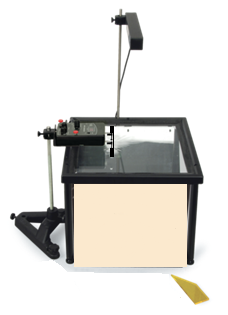
\includegraphics[width= 0.5 \linewidth]{IMAGENES/images/image9.png}
	\begin{tikzpicture}[>=latex, scale=0.9]
		\node (tmp) {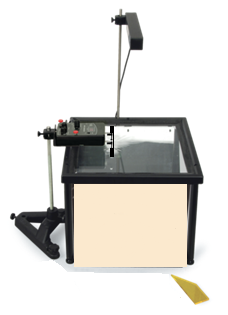
\includegraphics[width= 0.45 \linewidth]{IMAGENES/images/image9.png}};
		\draw [->, very thick ] (-5,1) node [left, text width=1.8cm] {Generador de Ondas} --++ (2,0);
		\draw [->, very thick] (-5,-4) node [left, text width=2.5cm] {Pantalla de Proyección} -- (-1,-3);
		\draw [->, very thick] (4,3) node [right] {Fuente de Luz} -- (1,4);
		\draw [->, very thick] (4,1.2) node [right] {Tanque} -- (2.5,1.2);
		\draw [->, very thick] (4,-1) node [right] {Reflector (por dentro)} -- (1,0.5);
		\draw [->, very thick] (4,-5) node [right, text width=3cm] {Pieza usada para obtener \(F_A\)} --++ (-1,0);
	\end{tikzpicture}
	\caption{Cuba de Ondas y Generador de Ondas usados en el expermento.}
	\label{fig_1}
\end{figure}
\newpage
\setuldepth{determinar}
Dado que \ul{se requiere determinar}, mediante el uso de la cuba, \ul{la velocidad de propagación} de la onda en el agua, procedimos obteniendo valores de los parámetros que nos ayudaron a tener los mínimos requeridos que la describen. \\[2mm]
En primera instancia lo que nos interesó fue encontrar la manera de relacionar la longitúd de onda con la frecuencia, para ello nos dimos cuenta de la ecuación, para ondas planas, que relaciona a tanto la longitúd como a la frecuencia mediante (\ref{velocidad}). \\[2mm]
Así, nos encontramos con la tarea de determinar los valores que nos ayuden a expresarlos. \\[2mm]
La propuesta que se dio (vía el manual) fue ajustar una recta respecto a ambas variables que, para una correcta dimensionalidad, la pendiente de dicha recta sería el período contra la longitud de onda para obtener la velocidad de la onda plana.
\[
	[v] = [\lambda] \cdot [f] = [\lambda] \cdot \dfrac{1}{[T]} = m \cdot \dfrac{1}{s} \mbox{.}
\]
Ahora, dado que la cuba de ondas proyecta franjas obscuras y luminosas fue necesario tener condiciones de luz muy bajas, externas al generador de ondas y a la fuente de luz,  como lo fue el sólo depender de la luz natural cerrando las ventanas aunque nos percatamos que una condición más ideal sería no tener luz, mejorando la calidad del enfoque de la proyección, y el usar un instrumento de medición que nos permita leer de manera digital el mensurando, pudiendo ser un vernier digital a diferencia del flexómetro utilizado,  siendo más precisa (cómoda para obtener) la medida dado que a ojo humano llegó a ser difícil incluso determinar en donde se generaban las franjas obscuras y luminosas de inicio a fin. \\[2mm]
Para calcular la longitud de onda, dado que se trabaja con una proyección, se tuvo que calcular el $F_A$, para ello usamos una pieza (reflectora) incluida con la cuba de ondas, pudiendo ser esta cualquiera siempre y cuando fuese fácil de poder manipularla por el usuario, de tal manera que se obtenga la longitud proyectada y la longitud real del objeto como se muestra a continuación en las Figuras \ref{fig_2} y \ref{fig_3}.
\begin{figure}[ht]
	\centering
	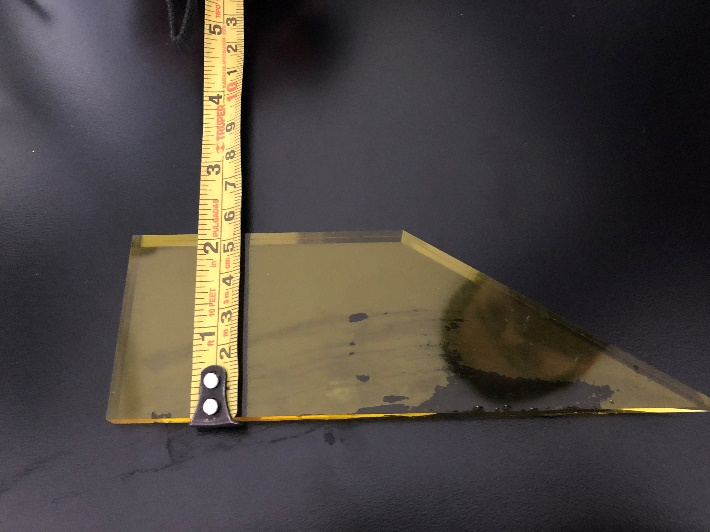
\includegraphics[height = 5.5cm]{IMAGENES/images/image1} \hspace{8mm}
	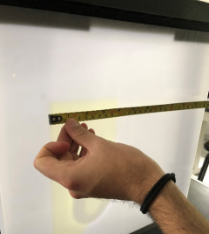
\includegraphics[height = 5.5cm]{IMAGENES/images/image8}
	\caption{Proceso de medición de la longitud real del objeto y la longitud proyectada del objeto respectivamente.}
	\label{fig_2}
\end{figure}\\
% \begin{figure}[ht]
	% \centering
	% 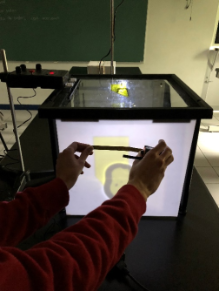
\includegraphics[width= 0.4 \linewidth]{IMAGENES/images/image3}% \caption{Visualización del proces de medición de la longitud proyectada del objeto junto con el objeto mismo sumergido parcialmente en el tanque.}
	% 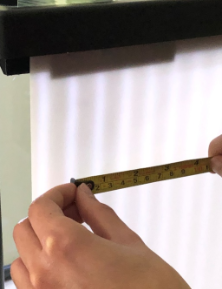
\includegraphics[width= 0.4 \linewidth]{IMAGENES/images/image2}% \caption{Proceso de medición de la longitud de iinda para una frecuencia y amplitud dada.}
	% \label{fig_3}
% \end{figure}\\
\begin{figure}
	\begin{minipage}{0.5\linewidth}
		\centering 
		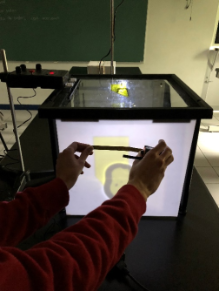
\includegraphics[height = 6cm]{IMAGENES/images/image3}
		\caption{Visualización del proceso de medición de la longitud proyectada del objeto junto con el objeto mismo sumergido parcialmente en el tanque.}
		\label{fig_3}
	\end{minipage}\hspace{8mm}
	\begin{minipage}{0.5\linewidth}
	\centering 
		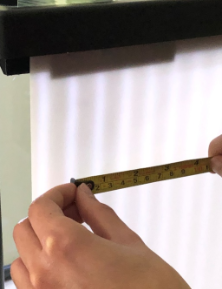
\includegraphics[height = 6cm]{IMAGENES/images/image2}
		\caption{Proceso de medición de la longitud de onda para una frecuencia y amplitud dada.}
		\label{fig_4}
		\vspace{1cm}
	\end{minipage}
\end{figure}
\newpage
Al obtener el valor $F_A$ proseguimos en obtener mediciones para la longitud de onda, variando las frecuencias, mediante lo obtenido al medir entre franja y franja obscura proyectada como se muestra en la Figura \ref{fig_4}. \\[2mm]
Para obtener el período, o en su efecto la frecuencia, se utilizó un cronometro, pues por definición del período, se buscaba el tiempo que tarda en transcurrir una onda, o a lo que es proporcional, el tiempo que tardan en transcurrir $n$ ondas de tal manera que a partir de aquí se consigue obtener las longitudes de onda con sus respectivas frecuencias para obtener la velocidad.
\begin{figure}[ht]
	\centering
	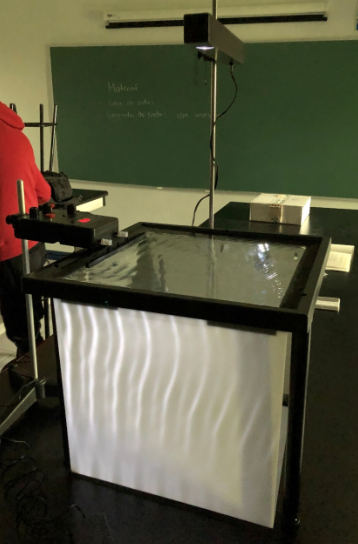
\includegraphics[height = 7cm]{IMAGENES/images/image5}
	\caption{Cuba de ondas en funcionamiento. En la pantalla de proyección se puede apreciar las franjas obscuras y luminosas relacionadas a las ondas que se fueron dando.}
\end{figure}
\newpage
% )))

\section{RESULTADOS.} % (((

\begin{itemize}[noitemsep]
	\item El instrumento de generación de ondas, tiene una incertidumbre de \(\pm 0.05Hz\).
	\item El instrumento de medición de longitudes, tiene una incertidumbre de \(\pm 0.05cm\).
	\item El instrumento de medición de tiempo, tiene una incertidumbre de \(\pm 0.005s\).
\end{itemize}

\subsection{--- Factor de Amplificación ---} % (((
\label{sub:factor_ampli}
Bajo la notación de la Sección \ref{caracteristicas}, se registra una medición de \(L ' = (10.2 \pm 0.05)cm\), y\\\(L = (5.1 \pm 0.05)cm\). Entonces, sustituyendo en la ecuación (\ref{factor_amplificacion}), se obtiene,
\[
	F_A = \dfrac{(10.2 \pm 0.05) cm}{(5.1 \pm 0.05) cm} = 2 \pm 0.03.
\]
Cuya incertidumbre está justificada en la Sección \ref{incertidumbres_4_1}.
% )))

\subsection{--- Frecuencia vs. Longitud de Onda ---} % (((
\label{sub:frecuencia_longitud_onda}
Se reporta en la Tabla \ref{primer_tabla}, siete frecuencias introducidas al generador de ondas, y sus respectivas mediciones de longitud de onda. A cada longitud se le aplicó el factor de re-escalamieto \(F_A\), y se muestra el tamaño real estimado. El cálculo de las incertidumbres se presenta en la Sección \ref{incertidumbres_4_2}.\\Se reporta en la fila \texttt{[Longitud de onda real]} la incertidumbre máxima obtenida en los datos.
\vspace{-6mm}
\begin{table}[ht]
	\centering 
	\caption{Medición de la longitud de onda a una frecuencia dada.}
	\begin{tabular}{|*{8}{l|}}
		\hline 
		% Medición &1 &2 &3 &4 &5 &6 &7 \\ \hline 
		Frecuencia (Hz) \(\pm 0.05Hz\) & 17 & 19 & 21 & 23 & 25 & 27 & 29 \\ \hline
		Longitud de onda proyectada \((cm) \pm 0.05cm\) &2.6  &2.5  &2.4  &2.1  &2    &1.7  &1.5 \\ \hline 
		Longitud de onda real \((cm)\) \(\pm 0.045cm\) &1.3  &1.25  &1.2  &1.05  &1    &0.85  &0.75 \\ \hline 
		% \(v=\lambda \cdot f\), (\(cm/seg\)) . &22.1	&23.75	&25.2	&24.15	&25	&22.95	&21.75 \\ \hline
	\end{tabular}
	\label{primer_tabla}
\end{table}
% )))

\subsection{--- Estimación de la Velocidad ---} % (((
\label{sub:calculo_velocidad}
En la Tabla \ref{segunda_tabla} se presentan cinco mediciones del tiempo transcurrido ante \(n=10\) frentes de onda (10 oscilaciones) a una frecuencia dada en las columnas \texttt{[T\(i\)]}, con \(i=1, \;\ldots,\; 5\). Se obtiene el promedio aritmético, de las cinco mediciones en la columna \texttt{[T. Prom.]}. En esta columna, se suman las incertidumbres de cada columna. El cálculo de la incertidumbre de las columnas \texttt{[Longitud de Onda]} y \texttt{[Frecuencia Estimada]} se encuentran en la Sección \ref{incertidumbres_4_3}. 
\begin{table}[ht]
	\footnotesize 
	\centering
	\caption{Tiempos obtenidos de diez oscilaciones a una frecuencia dada.}
	\begin{tabular}{|p{2cm}|*{5}{p{9mm}|}p{1.4cm}|p{2cm}|p{2.4cm}|}
		\hline 
		F. Real (\(Hz\)), & \multicolumn{5}{|c|}{Tiempo de 10 oscilaciones (\(seg\)), \(\pm 0.005s\).} & T. Prom.  & Longitud de & Frecuencia  \\ \cline{2-6}
		\(\pm 0.05Hz\). & T1 & T2 & T3 & T4 & T5 & (\(s\))\(\pm 0.025s\)&  Onda (\(cm\)).& Estimada (\(Hz\)).\\ \hline
		4 &2.52 &2.40 &2.24 &2.83 &2.67    &2.53    &6.5  \(\pm 0.12\) &3.95 \(\pm 0.04\) \\ \hline
		6 &1.62 &2.08 &1.97 &1.95 &2.03    &1.69    &3.2  \(\pm 0.07\) &5.91 \(\pm 0.09\) \\ \hline
		5 &1.38 &1.73 &1.72 &1.92 &1.74    &1.93    &4.25 \(\pm 0.09\) &5.18 \(\pm 0.07\) \\ \hline
		7 &		2.17 &2.14 &2.46 &2.38 &2.15 &2.26 &3.5  \(\pm 0.08\) &4.42 \(\pm 0.05\) \\ \hline
		8 &1.33 &1.42 &1.32 &1.37 &1.36    &1.36    &3.25 \(\pm 0.07\) &7.35 \(\pm 0.13\) \\ \hline
	\end{tabular}
	\label{segunda_tabla}
\end{table}
\newpage
En la Figura \ref{fig:lon_onda_vs_tiempo}, se colocan los datos de las columnas \texttt{[T. Prom.]} y \texttt{[Longitud de Onda]}. Para una escala útil, se esboza el eje \(10T\). Notamos que la ecuación (\ref{velocidad_2}) puede re-escribirse de la siguiente forma \vspace{-3mm}
\[
	v = \dfrac{\lambda}{T} = \dfrac{\Delta \lambda}{\Delta T}.
\]
Es decir, puede darse una estimación de la velocidad de las ondas a través de la pendiente de \(\lambda\) con respecto \(T\). En la Sección \ref{minimos_cuadrados_4_3} se realiza la estimación de la recta de regresión, la cuál, fue obtenida con los datos \((10T_i, \lambda _i)\). La recta tiene la siguiente pendiente.\vspace{-3mm}
\[
	a = \dfrac{\Delta \lambda}{\Delta 10T} = 2.2836 cm/s.
\]
Su respectivo análisis dimensional está justificado en la Sección \ref{sub:analisis_dim}. Tenemos que la estimación de la velocidad de las ondas planas en el agua es de
\[
	v = \dfrac{\Delta \lambda}{\Delta T} = 10a= 22.83cm/s.
\]
Se presenta la incertidumbre generada por el error estándar de \(\pm 11.2cm/s\), el cual, proviene de los datos experimentales \((10T_i, \lambda _i)\). El error, es obtenido en la Sección \ref{minimos_cuadrados_4_3}.
\[
	\fbox{\(v = (22.83 \pm 11.2) cm/s\).}
\]
\vspace{-1cm}
\begin{figure}[ht]
	\centering
	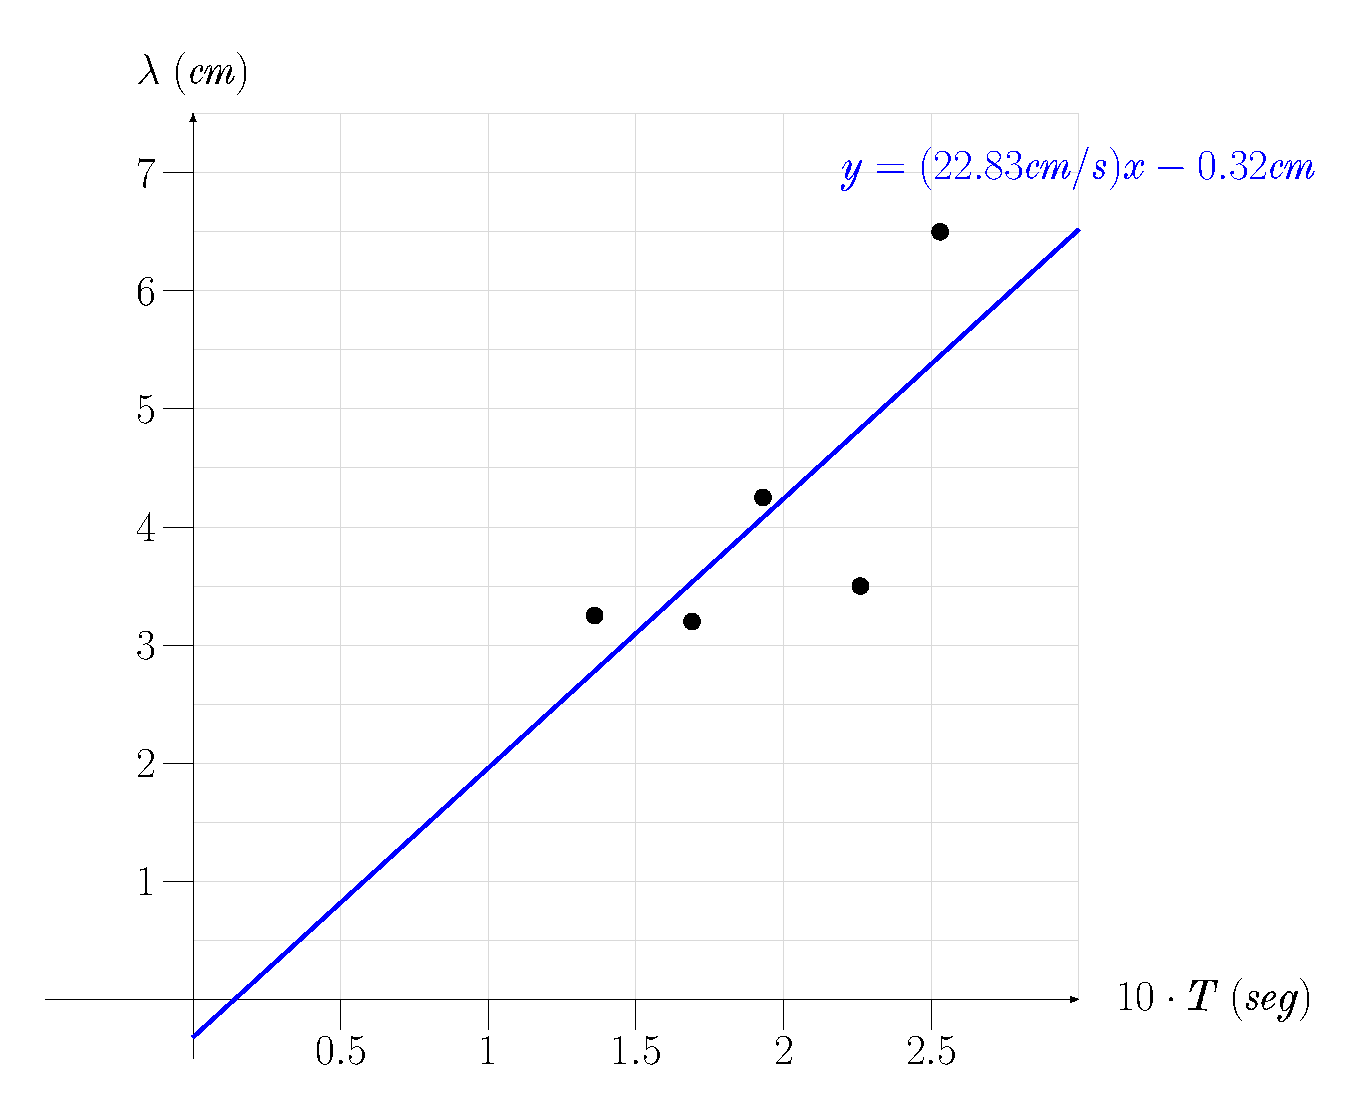
\includegraphics[height = 12cm]{IMAGENES/SECCION_4_3/tikz.pdf}
	\caption{Longitud de Onda vs Tiempo Promedio.}
	\label{fig:lon_onda_vs_tiempo}
\end{figure}
\newpage
% )))

\subsection{--- Errores en la Frecuencia ---} % (((
\label{sub:errores}
Se comparan las columnas \texttt{[Frecuencia Real]} y \texttt{[Frecuencia Estimada]} de la Tabla \ref{segunda_tabla} para observar el porcentaje de sus diferencias, en la columna \texttt{[Error relativo]} de la Tabla \ref{tercer_tabla}.
\begin{table}[ht]
	\centering
	\caption{Errores de medición de la Frecuencia.}
	\begin{tabular}{|p{3cm} |p{3.5cm} |p{2.5cm} |p{2.5cm}|}
		\hline 
		Frecuencia Real (\(Hz\)), \(\pm 0.05Hz\) & Frecuencia Estimada (\(Hz\)). & Error absoluto (\(Hz\)) & Error relativo \\ \hline
		4 & 3.95 \(\pm 0.04Hz\) & 0.05 \(\pm 0.09\) &1\textsc{\%}\\ \hline
		5 & 5.91 \(\pm 0.09Hz\) & 0.91 \(\pm 0.14\) &18\textsc{\%}\\ \hline
		6 & 5.18 \(\pm 0.07Hz\) & 0.82 \(\pm 0.12\) &14\textsc{\%}\\ \hline
		7 & 4.42 \(\pm 0.05Hz\) & 2.58 \(\pm 0.1\) &37\textsc{\%}\\ \hline
		8 & 7.35 \(\pm 0.13Hz\) & 0.65 \(\pm 0.18\) &8\textsc{\%}\\ \hline
	\end{tabular}
	\label{tercer_tabla}
\end{table}
% )))

% )))

\section{DISCUSIÓN DE RESULTADOS Y CONCLUSIONES.} % (((
Después de haberse producido las ondas con el generador proyectándose sobre la pantalla y así obtener tanto las mediciones de longitud de onda como las del tiempo de oscilaciones, fue posible determinar la velocidad de las ondas en el medio líquido. Esto gracias a la relación que existe entre la longitud de onda $\lambda$ y frecuencia $f$, que ésta última a su vez es el recíproco del período $T$, y viceversa. \\[2mm]
En la columna de \texttt{[Frecuencias Estimadas]} de la Tabla \ref{tercer_tabla}, se obtuvo que los errores en tres de las mediciones fueron menores al $15$\textsc{\%}, lo que entonces respalda la fórmula teórica entre la frecuencia y período mediante el cálculo de los recíprocos. En cambio, las otras dos mediciones tienen errores del $18$\textsc{\%} y $37$\textsc{\%}, lo que sólo podría justificarse mediante imprecisiones al hacer las mediciones. \\[2mm]
Los principales factores de ruido fueron: la iluminación en el laboratorio, debido a la cantidad de luz natural y artificial que perturbó la proyección de la onda del experimento; el otro provenía de nuestro instrumento para medir longitudes (flexómetro) junto con la forma en que se midieron las longitudes de onda, puesto que al hacer la medición sobre la pantalla no se puede colocar el flexómetro exactamente en donde comienza la franja, además de que el ángulo (perspectiva) desde el que se estaba midiendo también influyó al momento de obtener dicha medición. Este error pudo haberse evitado usando instrumentos de medición con una menor incertidumbre. \\[2mm]
Para el cálculo de la velocidad, luego de haberse obtenido las longitudes de onda con sus respectivos períodos, la recta estimada estadísticamente mediante el método de mínimos cuadrados concluye que las ondas generadas en el agua se mueven aproximadamente a una velocidad de $22.83\dfrac{cm}{s}$. El error (estadístico) obtenido para tal velocidad fue de $11.29\dfrac{cm}{s}$ y se atribuyen a las imprecisiones de medición ya mencionadas. \\[2mm]
Además, como se observa el la Figura \ref{fig:lon_onda_vs_tiempo}, conforme aumenta el período de oscilación, la longitud de la onda aumenta proporcionalmente a razón de la velocidad de la onda en el medio de propagación (el agua), puesto que conforme aumenta la longitud de onda un elemento en ella tardará más tiempo en recorrer tal longitud. Así pues, con este experimento se ha observado cómo el medio en donde se propaga la onda mecánica afecta a la velocidad en la que se mueve, lo que además justifica que una onda mecánica no podría transmitirse en el vacío porque no existe un elemento físico por el cual pueda avanzar. \\[2mm]
Así pues, verificamos experimentalmente la relación lineal que existe entre la velocidad, la longitud de onda y la frecuencia, descrita en la ecuación (\ref{velocidad}), con ondas mecánicas planas, realizando perturbaciones en el agua.
% )))

% === REFERENCIAS === (((
\bibliography{Referencias}
\bibliographystyle{unsrt}
% )))

\section{APÉNDICE.} % (((

\subsection{--- Incertidumbres de la Sección 4.1 ---} % (((
\label{incertidumbres_4_1}
Consúltese \([\)\cite{incert}\(]\), para la deducción de la ecuación (\ref{cociente_incert}). Si \(x,y \in \mathds{R}\), con \(x,y \ne 0\), son mediciones experimentales y \(\delta x, \delta y>0\) sus respectivas incertidumbres, entonces la incertidumbre del cociente \(q = x/y\), está dada por
\begin{equation}
	\dfrac{\delta q}{|q|} = \dfrac{\delta x}{|x|} + \dfrac{\delta y}{|y|}.
	\label{cociente_incert}
\end{equation}
es decir,
\[
	\delta q = \left| \dfrac{x}{y} \right| \dfrac{\delta x}{|x|} + \left| \dfrac{x}{y} \right| \dfrac{\delta y}{|y|}.  
\]
y por tanto,
\begin{equation}
	\dfrac{x\pm \delta x}{y\pm \delta y} = \dfrac{x}{y} \pm \Bigg(\dfrac{\delta x}{|y|} + |x|\dfrac{\delta y}{|y|^2}\Bigg).
	\label{eq:calculo_incert}
\end{equation}
Entonces, sustituyendo en la ecuación (\ref{factor_amplificacion}), se tiene
\begin{equation}
		F_A=\dfrac{(10.2 \pm 0.05) cm}{(5.1 \pm 0.05) cm} = \dfrac{10.2}{5.1} \pm \Bigg(\dfrac{0.05}{5.1} + 10.2\dfrac{0.05}{5.1^2}\Bigg) = 2 \pm 0.03
	\label{eq:factor_resc}
\end{equation}
% )))

\newpage
\subsection{--- Incertidumbres de la Sección 4.2 ---} % (((
\label{incertidumbres_4_2}
Usando la ecuación (\ref{eq:calculo_incert}), y el factor de escalamiento \(F_A\), de la ecuación (\ref{eq:factor_resc}), se tienen los siguientes resultados para la fila \texttt{[Longitud de Onda Real]}, de la Tabla \ref{primer_tabla}.
\[
	\begin{array}{rcl}
		\dfrac{(2.6 \pm 0.05)cm}{2\pm 0.03} & = & 1.3cm \pm  \Bigg(\dfrac{0.05}{2} + 2.6\dfrac{0.03}{2^2}\Bigg)cm = ( 1.3 \pm 0.044)cm \\[6mm]
		\dfrac{(2.5 \pm 0.05)cm}{2\pm 0.03} & = & 1.25cm \pm \Bigg(\dfrac{0.05}{2} + 2.5\dfrac{0.03}{2^2}\Bigg)cm = (1.25 \pm 0.043)cm \\[6mm]
		\dfrac{(2.4 \pm 0.05)cm}{2\pm 0.03} & = & 1.2cm \pm  \Bigg(\dfrac{0.05}{2} + 2.4\dfrac{0.03}{2^2}\Bigg)cm =  (1.2 \pm 0.043)cm \\[6mm]
		\dfrac{(2.1 \pm 0.05)cm}{2\pm 0.03} & = & 1.05cm \pm \Bigg(\dfrac{0.05}{2} + 2.1\dfrac{0.03}{2^2}\Bigg)cm = (1.05 \pm 0.041)cm \\[6mm]
	\end{array}
\]
\[
	\begin{array}{rcl}
		\dfrac{(2 \pm 0.05)cm}{2\pm 0.03} & = & 1cm \pm    \Bigg(\dfrac{0.05}{2}   + 2  \dfrac{0.03}{2^2}\Bigg)cm =    (1 \pm 0.04)cm \\[6mm]
		\dfrac{(1.7 \pm 0.05)cm}{2\pm 0.03} & = & 0.85cm \pm \Bigg(\dfrac{0.05}{2} + 1.7\dfrac{0.03}{2^2}\Bigg)cm = (0.85 \pm 0.038)cm \\[6mm]
		\dfrac{(1.5 \pm 0.05)cm}{2\pm 0.03} & = & 0.75cm \pm \Bigg(\dfrac{0.05}{2} + 1.5\dfrac{0.03}{2^2}\Bigg)cm = (0.75 \pm 0.036)cm
	\end{array}
\]
% )))

\subsection{--- Incertidumbres de la Sección 4.3. ---} % (((
\label{incertidumbres_4_3}
Se usa nuevamente la ecuación (\ref{eq:calculo_incert}) y el factor \(F_A\) de la ecuación (\ref{eq:factor_resc}), para obtener las estimaciones de la columna \texttt{[Longitud de Onda]} de la Tabla \ref{segunda_tabla}. 
\[
	\begin{array}{rcl}
		\dfrac{(13 \pm 0.05)cm}{2 \pm 0.03} & = & 6.5cm  \pm \Bigg(\dfrac{0.05}{2}  + 13 \dfrac{0.03}{2^2}\Bigg) =    (6.5 \pm 0.122)cm \\[6mm]
		 \dfrac{(6.4 \pm 0.05)cm}{2 \pm 0.03} & = & 3.2cm  \pm \Bigg(\dfrac{0.05}{2} + 6.4\dfrac{0.03}{2^2}\Bigg) =   (3.2 \pm 0.073)cm \\[6mm]
		 \dfrac{(8.5 \pm 0.05)cm}{2 \pm 0.03} & = & 4.25cm \pm \Bigg(\dfrac{0.05}{2} + 8.5\dfrac{0.03}{2^2}\Bigg) =  (4.25 \pm 0.088)cm \\[6mm]
			 \dfrac{(7 \pm 0.05)cm}  {2 \pm 0.03} & = & 2.5cm  \pm \Bigg(\dfrac{0.05}{2}   + 7  \dfrac{0.03}{2^2}\Bigg)=(3.5 \pm 0.077)cm \\[6mm]
		 \dfrac{(6.5 \pm 0.05)cm}{2 \pm 0.03} & = & 3.25cm \pm \Bigg(\dfrac{0.05}{2} + 6.5\dfrac{0.03}{2^2}\Bigg) =  (3.25 \pm 0.073)cm \\[6mm]
	\end{array}
\]
% Ahora, para obtener la incertidumbre de la columna \texttt{[Frecuenia Estimada]} de la Tabla \ref{segunda_tabla}, se tomará a \(x=10\) y \(\delta x=0\), en la ecuación (\ref{eq:calculo_incert}), para obtener el recíproco de la columna \texttt{[T. Prom.]} multiplicado por \(10\).
% Esto es debido a que se registró \(10T\) en cada columna \texttt{T\(i\)}, al obtener el promedio se tiene una estimación de \(10T\), es decir, 10 períodos de oscilación. Y \(f= \dfrac{1}{T} = \dfrac{10}{10T}\), y \(10T\) es la cantidad medida.
Ahora, se requiere obtener la incertidumbre de la columna \texttt{[Frecuencia Estimada]} de la Tabla \ref{segunda_tabla}. Para ello, notamos que la ecuación (\ref{eq:frecuencia}) puede escribirse como, \(f= \dfrac{1}{T} = \dfrac{10}{10T}\), y que el numerador es adimensional y por tanto, tiene incertidumbre cero. Así, se usa la ecuación (\ref{cociente_incert}), con \(x=10\), \(\delta x=0\), \(y=10T_i\), en las siguientes incertidumbres.
\[
	\begin{array}{rcl}
		\dfrac{10 \pm 0}{2.53s \pm 0.025s} & = & 3.95Hz \pm \Bigg(\dfrac{0}{2.53} + 10 \dfrac{0.025}{2.53^2}\Bigg) = (3.95 \pm 0.039)Hz \\[6mm]
		\dfrac{10 \pm 0}{1.69s \pm 0.025s} & = & 5.91Hz \pm \Bigg(\dfrac{0}{1.69} + 10 \dfrac{0.025}{1.69^2}\Bigg) = (5.91 \pm 0.087)Hz \\[6mm]
		\dfrac{10 \pm 0}{1.93s \pm 0.025s} & = & 5.18Hz \pm \Bigg(\dfrac{0}{1.93} + 10 \dfrac{0.025}{1.93^2}\Bigg) = (5.18 \pm 0.067)Hz \\[6mm]
		\dfrac{10 \pm 0}{2.26s \pm 0.025s} & = & 4.42Hz \pm \Bigg(\dfrac{0}{2.26} + 10 \dfrac{0.025}{2.26^2}\Bigg) = (4.42 \pm 0.048)Hz \\[6mm]
		\dfrac{10 \pm 0}{1.36s \pm 0.025s} & = & 7.35Hz \pm \Bigg(\dfrac{0}{1.36} + 10 \dfrac{0.025}{1.36^2}\Bigg) = (7.35 \pm 0.135)Hz
	\end{array}
\]
% Consúltese (referencia: incertidumbres) si \(x,y \in \mathds{R}\) son mediciones, y \(\delta x, \delta y>0\) son sus respectivas incertidumbres, entonces
% \[
	% \delta (xy) = |y|\delta x+ |x| \delta y.
% \]
% Finalmente, se requiere obtener la incertidumbre de la velocidad estimada. Sean \((T_i, \lambda _i)\) los datos experimentales del período y la longitud de onda respectivamente. Sean \(\delta T, \delta \lambda >0\), sus incertidumbres máximas. Entonces
% \[
	% a = \dfrac{n \dis\suma_{i=1}^{n} T_i \lambda _i - \Bigg(\dis\suma_{i=1}^{n} T_i\Bigg) \Bigg(\dis\suma_{i=1}^{n} \lambda _i\Bigg)}{n \dis\suma_{i=1}^{n} T_i ^2- \Bigg(\dis\suma_{i=1}^{n} \lambda _i\Bigg) ^2}
% \]
% requiere de un análisis para cada uno de los elementos de la expresión.
% \begin{enumerate}
	% \item[\fbox{Primer término}] 
		% \[
			% \begin{array}{rcl}
				% \dis\suma_{i=1}^{n} (T_i+ \delta T) (\lambda _i+ \delta \lambda) &=& \dis\suma_{i=1}^{n} (T_i \lambda _i+ \delta T \lambda _i+ \delta \lambda T_i) \\[2mm]
				% & \leqslant & \dis\suma_{i=1}^{n} T_i \lambda _i + n \delta T \cdot \max _i(\lambda _i) + n \delta \lambda \cdot \max _i(T_i).
			% \end{array}
		% \]
		% Así, \(n \dis\suma_{i=1}^{n} T_i \lambda _i\) tiene una incertidumbre acotada por \(n^2 \delta T \cdot \max _i(\lambda _i) + n^2 \delta \lambda \cdot \max _i(T_i)\).
	% \item[\fbox{Segundo término}] La incertidumbre de \(\dis\suma_{i=1}^{n} T_i\) es \(n \delta T\). Análigamente, la incetidumre de \(\dis\suma_{i=1}^{n} \lambda _i\) es \(n \delta \lambda\).\\Por lo tanto, la incertidumbre de su producto \(\Bigg(\dis\suma_{i=1}^{n} T_i\Bigg) \Bigg(\dis\suma_{i=1}^{n} \lambda _i\Bigg)\) es
		% \[
			% n\delta \lambda \Bigg(\dis\suma_{i=1}^{n} T_i\Bigg) + n\delta T \Bigg(\dis\suma_{i=1}^{n} \lambda _i\Bigg) \leqslant \delta \lambda \cdot n \max (T_i) + \delta T \cdot n \max (\lambda _i).
		% \]
% \end{enumerate}
% )))

\subsection{--- Análisis Dimensional de la Sección 4.3 ---} % (((
\label{sub:analisis_dim}
En la Figura \ref{fig:lon_onda_vs_tiempo} se tienen los pares ordenados \((10T_i, \lambda _i)\), donde \([10T_i] = s\), y \([\lambda _i] = cm\), por tanto, se sustituye en las ecuaciones (\ref{eq:intercept}).
\[
	\begin{array}{rcl}
		[a] & = & \dfrac{n \dis\suma_{i=1}^{n} [10T_i] [\lambda _i] - \Bigg(\dis\suma_{i=1}^{n} [10T_i]\Bigg) \Bigg(\dis\suma_{i=1}^{n} [\lambda _i]\Bigg)}{n \dis\suma_{i=1}^{n} [10T_i] ^2- \Bigg(\dis\suma_{i=1}^{n} [10T _i]\Bigg) ^2} \\[6mm]
		& = & \dfrac{s \cdot cm - s \cdot cm}{s^2-s^2} \\[6mm]
		& = & \dfrac{s \cdot cm}{s^2} \\[6mm]
		& = & \dfrac{cm}{s}.
	\end{array}
\]
\[
	\begin{array}{rcl}
		[b] & = & \dfrac{\left(\dis\suma_{i=1}^n [10T_i]^2\right)\left(\dis\suma_{i=1}^n [\lambda_i]\right)-\left(\dis\suma_{i=1}^n [10T_i] \right)\left(\dis\suma_{i=1}^n [10T_i] [\lambda_i]\right) }{n \left(\dis\suma_{i=1}^n [10T_i]^2\right)-\left(\dis\suma_{i=1}^n [10T_i]\right)^2} \\[6mm] 
		& = & \dfrac{s^2 \cdot cm - s \cdot (s \cdot  cm)}{s^2-s^2} \\[6mm]
		& = & \dfrac{s^2 \cdot cm}{s^2} \\[6mm]
		& = & cm.
	\end{array}
\]
A su vez, se realizan las operaciones para verificar la dimensión de la varianza de los datos \((10T_i, \lambda _i)\). Consúltese \([\)\cite{mont}\(]\), para la justificación de la ecuación (\ref{eq:var}).
\begin{equation}
	\mbox{\textit{var}} (a) = \dfrac{\dfrac{1}{n} \dis\suma_{i=1}^{n} \big(\lambda _i - (a10T_i-b)\big) ^2}{\dis\suma_{i=1}^{n} (10T_i - \overline{10T}) ^2}.
	\label{eq:var}
\end{equation}
Entonces
\[
	\begin{array}{rcl}
		[\mbox{\textit{var}} (a)]  &=& \dfrac{\dfrac{1}{n} \dis\suma_{i=1}^{n} \big([\lambda_i] - ([a] \cdot [10T_i]-[b])\big) ^2}{\dis\suma_{i=1}^{n} ([10T_i] - [\overline{10T}]) ^2} \\[2mm]
		& = & \dfrac{\big[cm - cm/s \cdot s-cm\big] ^2}{s^2} \\[6mm]
		& = & \dfrac{cm^2}{s^2}.
	\end{array}
\]
Así, el error estándar, \(\widehat{\sigma} = \sqrt{\mbox{\textit{var} (a)}} \), tiene unidades \(cm/s\).
% )))

\subsection{--- Mínimos Cuadrados de la Sección 4.3. ---} % (((
\label{minimos_cuadrados_4_3}
Se almacenan las columnas \texttt{[T. Prom.]} y \texttt{[Longitud de Onda]} de la Tabla \ref{segunda_tabla}, en el archivo \texttt{[datos2.txt]}
\begin{lstlisting}[backgroundcolor = \color{gray!13}]
Tiempo Long_Onda
2.53 6.5
1.69 3.2
1.93 4.25
2.26 3.5
1.36 3.25
	\end{lstlisting}
	Se obtiene la recta de regresión, con el software \texttt{R}, el cual emplea el método de mínimos cuadrados de la siguiente manera.
	\begin{lstlisting}
library(lmtest)
datos = read.table('datos2.txt', header = TRUE) 
regresion = lm(Long_Onda~Tiempo,data=datos)
regresion$coefficients
	\end{lstlisting}
Reporta el siguiente resultado.
\begin{lstlisting}[backgroundcolor = \color{gray!13}]
(Intercept)      Tiempo 
 -0.3221998   @@2.2836232@@
\end{lstlisting}
Se denota en verde, al coeficiente que indica la pendiente de la recta. \\[2mm]
Ahora, recordemos que el error estándar de los valores \((10T_i,\lambda _i)\), mide la variabildad total de los datos con respecto a la recta de estimación, así como lo indica la expresión (\ref{eq:var}). \\[2mm]
Para su obtención se usa el siguiente comando.
\begin{lstlisting}
summary(regresion)$coefficients
\end{lstlisting}
Obteniéndose un error estándar de \texttt{[1.12 \(cm/s\)]}, en la pendiente de los datos. (Su análisis dimensional está justificado en la Sección \ref{sub:analisis_dim}).
\begin{lstlisting}[backgroundcolor = \color{gray!13}]
              Estimate Std. Error    t value  Pr(>|t|)
(Intercept) -0.3221998   2.253638 -0.1429688 0.8953774
Tiempo       2.2836232   @1.128539@  2.0235226 0.1361922
\end{lstlisting}
% )))

% )))

\end{document}
